\chapter{METODOLOGIA}

%Metodologia da bibliografia
\section{Metodologia usada no Levantamento Bibliográfico}

Para atingir os objetivos que orientam este estudo, os procedimentos metodológicos foram planejados tendo como base programas educacionais que visam a promoção do empreendedorismo e comportamento empreendedor na condução dos cursos de graduação, em instituições de ensino públicas e particulares, como também Startups de natureza educacional.


\section{Programa Empreenda AGRO Sustentável: considerações metodológicas}


As atividades serão desenvolvidas por meio de quatro Workshops, que constam metodologias ativas, oficinas, palestras, e ferramentas tecnológicas visando à sinergia entre as estratégias de inovação no uso de tecnologias educacionais e os objetivos da proposta, com vistas a promover aprendizagem significativa e colaborativa. Todas as etapas do projeto de pesquisa serão planejadas e executadas utilizando a metodologias ativas, objetivando o aprendizado do uso das ferramentas de gestão e planejamento de empreendimentos.
Durante os módulos do projeto (Workshops), os participantes testarão de seus projetos para que novas requisições sejam realizadas e/ou que erros nos planejamentos sejam encontrados e, consequentemente, debatidos e mitigados, utilizando para isso os métodos de modelagem de negócio (Lean Canvas e Business Model Canvas). Depois que todas as Sprints (atividades dos três Workshops) forem finalizadas, ou seja, que todos os módulos forem trabalhados, será iniciado um ciclo de Apresentações e desenvolvimento da habilidade de apresentação e demonstração dos produtos por meio de apresentações (\textit{Pitch}). Destaca-se, ainda, que as inovações passiveis de registro intelectual apresentadas nesta pesquisa serão incentivadas a registro e documentação dos direitos.


\newpage
\subsection{Planejamento}

Com a finalidade de propor uma melhor mentoria no desenvolvimento dos objetivos propostos, o programa será desenvolvido em quatro encontros (Workshops), que abordarão temas pertentes ao empreendedorismo e o comportamento empreendedor, a saber:

\begin{itemize}
\item{1\textsuperscript{o} Workshop - Serão abordados os seguintes temas: O que é Startups, Empreendedorismo, comportamento empreendedor e cultura empreendedora, Problemas (segmentação do mercado), segundo os Objetivos do Desenvolvimento Sustentável (ODS), Modelagem do negócio e Criatividade}

\item{2\textsuperscript{o} Workshop - Serão abordados os seguintes temas: A busca de oportunidades como Característica Empreendedora, Construção do Lean Canvas, Mapa de Empatia, Validação da Proposta de Valor e Economia colaborativa e Coworking}
\item{3\textsuperscript{o} Workshop - Serão abordados os seguintes temas: Hackathon: Prototipagem para o MVP, O que você pode fazer por seu cliente e como o cliente adquire seu produto?}
\item{4\textsuperscript{o} Workshop - Serão abordados os seguintes temas: Pitch e o Demoday}

\end{itemize}

\subsection{Mobilização das equipes:}

Inicialmente serão abertas vagas para estudantes do curso de graduação ligadas aos cursos de Ciências Agrárias da Universidade Federal de Sergipe-UFS, onde as inscrições serão realizadas por equipe, desde que preencham os seguintes critérios:

	
\begin{itemize}
\item{Estarem regularmente matriculados e cursando quaisquer dos cursos e ao menos um aluno ligado as ciências agrárias;}
\item{Comprovarem disponibilidade de tempo para participação em todas as oficinas programadas;}
\item{Lidar com trabalhos em equipe.}
\end{itemize}

Objetiva-se o alcance de \textbf{120 alunos} participantes efetivos no programa, o qual será considerado o número de amostra para o estudo. 

\newpage
\section{Questionário para análise de Campo}

A pesquisa será desenvolvida com caráter descritivo, uma vez que busca analisar o potencial do comportamento empreendedor e a competências Empreendedoras, dos acadêmicos dos cursos de graduação em Ciências Agrárias inscritos no Programa Empreenda AGRO Sustentávely, utilizando como fator indutor para melhoria o programa de extensão Empreenda Agro Sustentável a partir do modelo \textit{Global University Entrepreneurial Spirit Students’ Survey} (GUESSS), conhecido nacionalmente por Estudo GUESSS. Esta ferramenta de estudo busca caracterizar o espírito, as atividades e as intenções empreendedores de estudantes universitários, de todos os níveis de estudo e em todos os cursos universitários, bem como as condições de ensino e apoio a atividades empreendedoras. 




Por critérios éticos o questionário aplicado nesta pesquisa atende os termos das Resolução n. 466 de 12 de dezembro de 2012 do Conselho Nacional de Saúde \cite{cns_resolucao_2012}, o qual por se tratar de pesquisa com seres humanos foi submetido ao Comitê de Ética em Pesquisa Envolvendo Seres Humanos (\textbf{CEP}) e a Comissão Nacional de Ética em Pesquisa (\textbf{Conep}) por meio da plataforma Brasil Saúde tendo como Certificado de Apresentação para Apreciação Ética \textbf{CAAE: 23853219.4.0000.5546}. O questionário apresenta 5 conjuntos de questões dos mais diversos contextos relacionados ao empreendedorismo, medindo diferentes elementos do empreendedorismo e comportamento empreendedor no meio educacional tanto vindo dos discentes quanto dos docentes. Destaca-se que o instrumento de pesquisa que será utilizado neste experimento foi composto por Cinco blocos de questões de múltipla escolha baseadas principalmente em escalas de cinco ou sete possibilidades. 

O primeiro conjunto de questões está relacionado a informações que buscam traçar o perfil dos alunos entrevistados, tais como: gênero, faixa etária, curso vinculado e o perfil de interesse nas áreas de estudo ligadas ao empreendedorismo sustentável tal questionário foi baseado no trabalho desenvolvido por \citeonline{lima_educacao_2014}. 

O segundo bloco e composto por 10 questões relacionadas a auto eficácia dos estudantes de múltipla escolha partindo da alternativa “Completamente Inseguro” a Completamente Seguro”. 

O terceiro bloco e composto por 7 questões que analisam a intenção empreendedora do aluno da quais segue uma proporção partindo da resposta, tendo como alternativas partido do “Discordo totalmente” a “Concordo totalmente”.

O Quarto bloco retrata a intenção em ter sua própria empresa ou ser autônomo e por fim o Quinto bloco contendo 11 questões abordará a ligação da família e o apoio familiar no empreendedorismo, tendo como alternativas partido do “Discordo totalmente” a “Concordo totalmente”. 

Esta pesquisa apresenta uma população de 1.453 discentes dos cursos de graduação nas áreas de agrárias da Universidade Federal de Sergipe (UFS): Engenharia Agronômica, Engenharia Agrícola, Zootecnia, Engenharia Florestal, Medicina Veterinária e Engenharia de Pesca, dados contidos no relatório estatístico de matriculas 2017 da instituição, \cite{campelo_ufs_2018}. É importante levar em conta que este estudo não levou em consideração classe social local de estudo anterior, e desempenho acadêmico do aluno durante a graduação. 
A amostra compreenderá 120 discentes que participarem do Programa Empreenda Agro Sustentável que responderão os questionários instrumento de pesquisa que serão aplicados durante os Workshops. Tais Workshops ocorrerão nos meses de agosto, outubro e novembro de 2019. Tal instrumento será aplicado presencialmente. O estudo caracteriza-se como uma pesquisa de levantamento ou \textit{Survey} do tipo Descritivo sob corte Longitudinal, que segundo \citeonline{tormen_potencial_2005} destaca-se por compreender uma amostra expressiva em relação ao universo pesquisado na Figura \ref{figura_1} é possível compreender as fases de uma pesquisa tipo \textit{Survey}.

\begin{figure}[!htb]
\centering
\caption{\textbf{Fases da pesquisa Survey}}
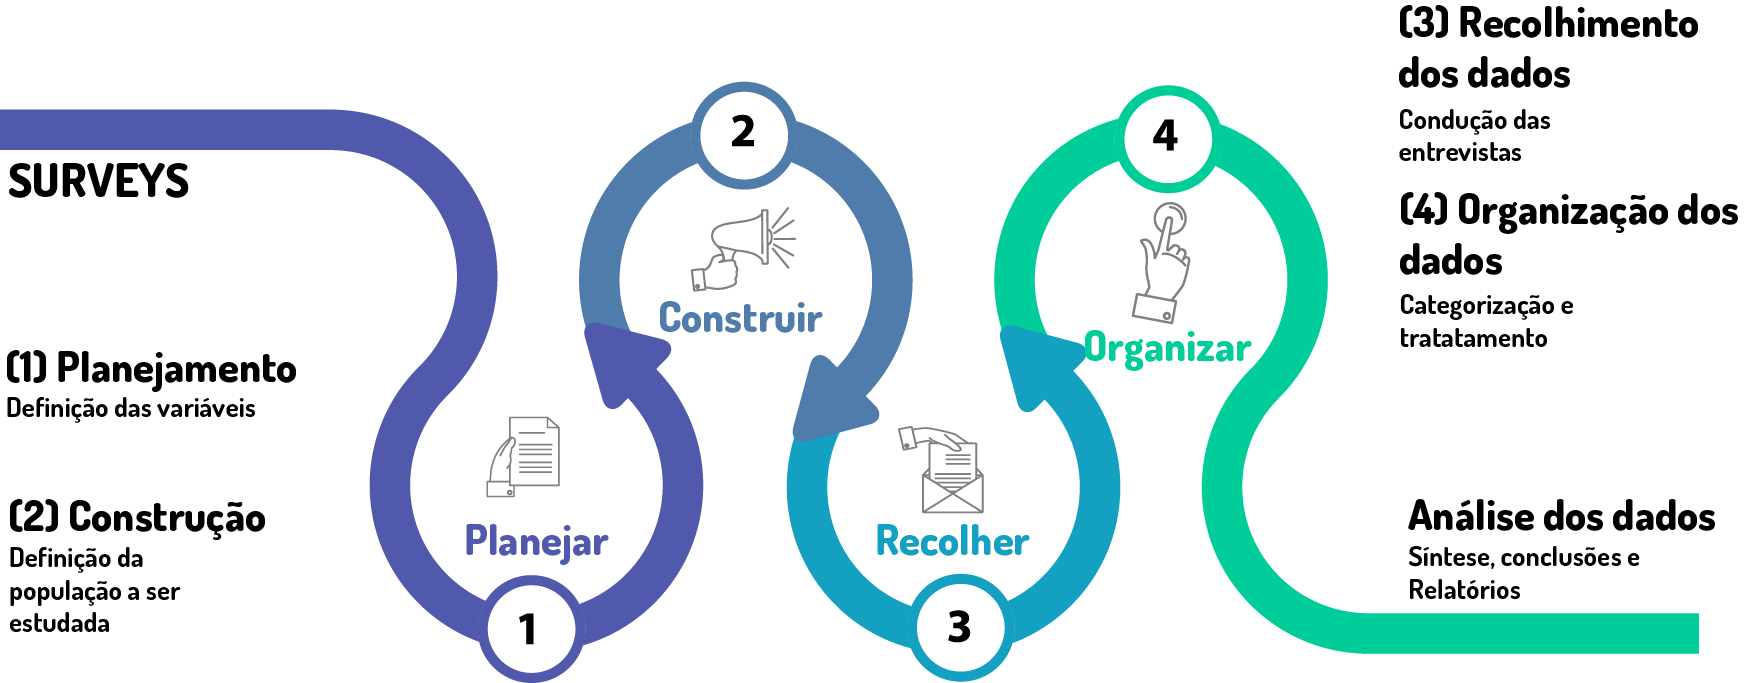
\includegraphics[scale=0.5]{Imagens/diagrama_survey.png}
\fonte{Adaptado de \cite{moser_survey_2017}}
\label{figura_1}
\end{figure}


\clearpage


%estatística
\section{Análises Estatísticas}

Para o processamento dos dados será utilizado o Software Rstudio \cite{rstudio_team_rstudio:_2015}. A avaliação da normalidade dos dados utilizado será analisada através do teste de Normalidade kolmogorov-smirnov (K-S) a (p> 0,05),  \cite{da_cunha_nascimento_testes_2017}. Caso os resultados apresentem distribuição normal, será utilizado o teste paramétrico de hipótese ANOVA com nível de significância de 0,05.


\begin{landscape}
\section{Cronograma}
\begin{ganttchart}[
canvas/.append style={fill=none, draw=black!5, line width=.75pt},
hgrid style/.style={draw=black!5, line width=.75pt},
vgrid={*1{draw=black!5, line width=.75pt}},
today=12,
today rule/.style={
draw=black!64,
dash pattern=on 3.5pt off 4.5pt,
line width=1.5pt
},
today label font=\small\bfseries,
title/.style={draw=none, fill=none},
title label font=\bfseries\footnotesize,
title label node/.append style={below=7pt},
include title in canvas=false,
bar label font=\mdseries\small\color{black!70},
bar label node/.append style={left=2cm},
bar/.append style={draw=none, fill=black!63},
bar incomplete/.append style={fill=barblue},
bar progress label font=\mdseries\footnotesize\color{black!70},
group incomplete/.append style={fill=barblue},
group left shift=0,
group right shift=0,
group height=.5,
group peaks tip position=0,
group label node/.append style={left=.6cm},
group progress label font=\bfseries\small,
link/.style={-latex, line width=1.5pt, linkred},
link label font=\scriptsize\bfseries,
link label node/.append style={below left=-2pt and 0pt},
]{1}{25}
\gantttitle{Cronograma}{25} \\[grid]
\gantttitle{Agosto}{4}
\gantttitle{Setembro}{4}
\gantttitle{Outubro}{4}
\gantttitle{Novembro}{4}
\gantttitle{Dezembro}{4}
\gantttitle{Janeiro}{4}
\gantttitle{Fevereiro}{4}\\
\gantttitle[
title label node/.append style={below left=7pt and -3pt}
]{Semana:\quad1}{1}
\gantttitlelist{2,...,25}{1} \\
\ganttgroup[progress=50]{Projeto Dissertação}{1}{25} \\
\ganttbar[progress=100,name=bar1]{\textbf{Pesquisa do Estado da Arte}}{1}{5} \\
\ganttbar[progress=100,name=bar2]{\textbf{Delineamento da Pesquisa}}{2}{4} \\
\ganttbar[progress=100,name=bar3]{\textbf{Elaboração do Projeto de Pesquisa}}{4}{5} \\
\ganttbar[progress=100,name=bar5]{\textbf{Discussão Metodológica}}{5}{7} \\
\ganttbar[progress=50,name=bar4]{\textbf{Programa Experimento}}{5}{20} \\
\ganttbar[progress=00,]{\textbf{Aplicação dos testes}}{17}{20} \\\ganttbar[progress=00,]{\textbf{Análise dos resultados}}{20}{22}\\
\ganttmilestone{Qualificação}{24}{24}  \\
%\ganttmilestone{Hito 2}{12}{12} \\
\ganttbar[progress=00,]{\textbf{Correções solicitadas}}{25}{25} \\

%\ganttbar[progress=0,]{\textbf{Actividad 9}}{23}{24} \\

%\ganttmilestone{Q6 report}{24}{24} \\
\ganttmilestone{Defesa}{25}{25}

%\ganttlink[link type=f-s]{bar1}{bar2}
%\ganttlink[link type=f-s]{bar4}{bar5}
\end{ganttchart}
\end{landscape}